\documentclass{../template/myrpt}
\ExamName{热电偶的定标实验}
\newlist{experimentsteps}{enumerate}{1}
\setlist[experimentsteps,1]{
  label=\textbf{\arabic*.},
  leftmargin=0pt,
  labelsep=0pt,
  itemindent=0pt,
  align=left,
  topsep=0pt,
  partopsep=0pt,
  parsep=0pt,
  itemsep=0.75\baselineskip
}
\pgfplotsset{compat=1.18}

\begin{document}
\maketitle

\section{实验目的}
\begin{enumerate}[label=\arabic*. ]
  \item 了解热电偶测温的基本原理和方法；
  \item 了解热电偶的定标方法；
  \item 为热电偶定标。
\end{enumerate}

\section{实验仪器}

\begin{figure}[htbp]
  \centering
  \begin{minipage}[c]{0.42\linewidth}
    \centering
    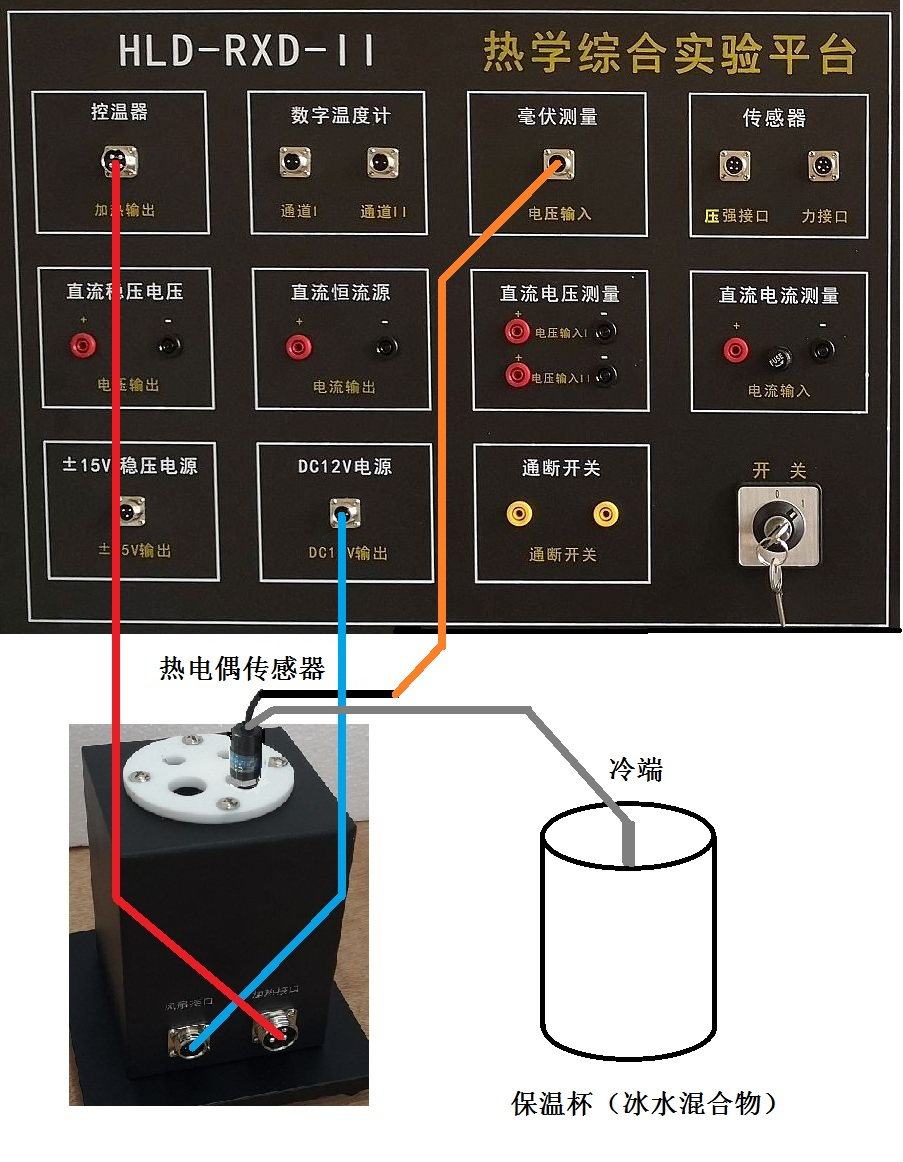
\includegraphics[width=\linewidth]{assets/接线图.jpeg}
    \caption{实验接线图}
  \end{minipage}
  \hspace{1em}
  \begin{minipage}[c]{0.5\linewidth}
    \centering
    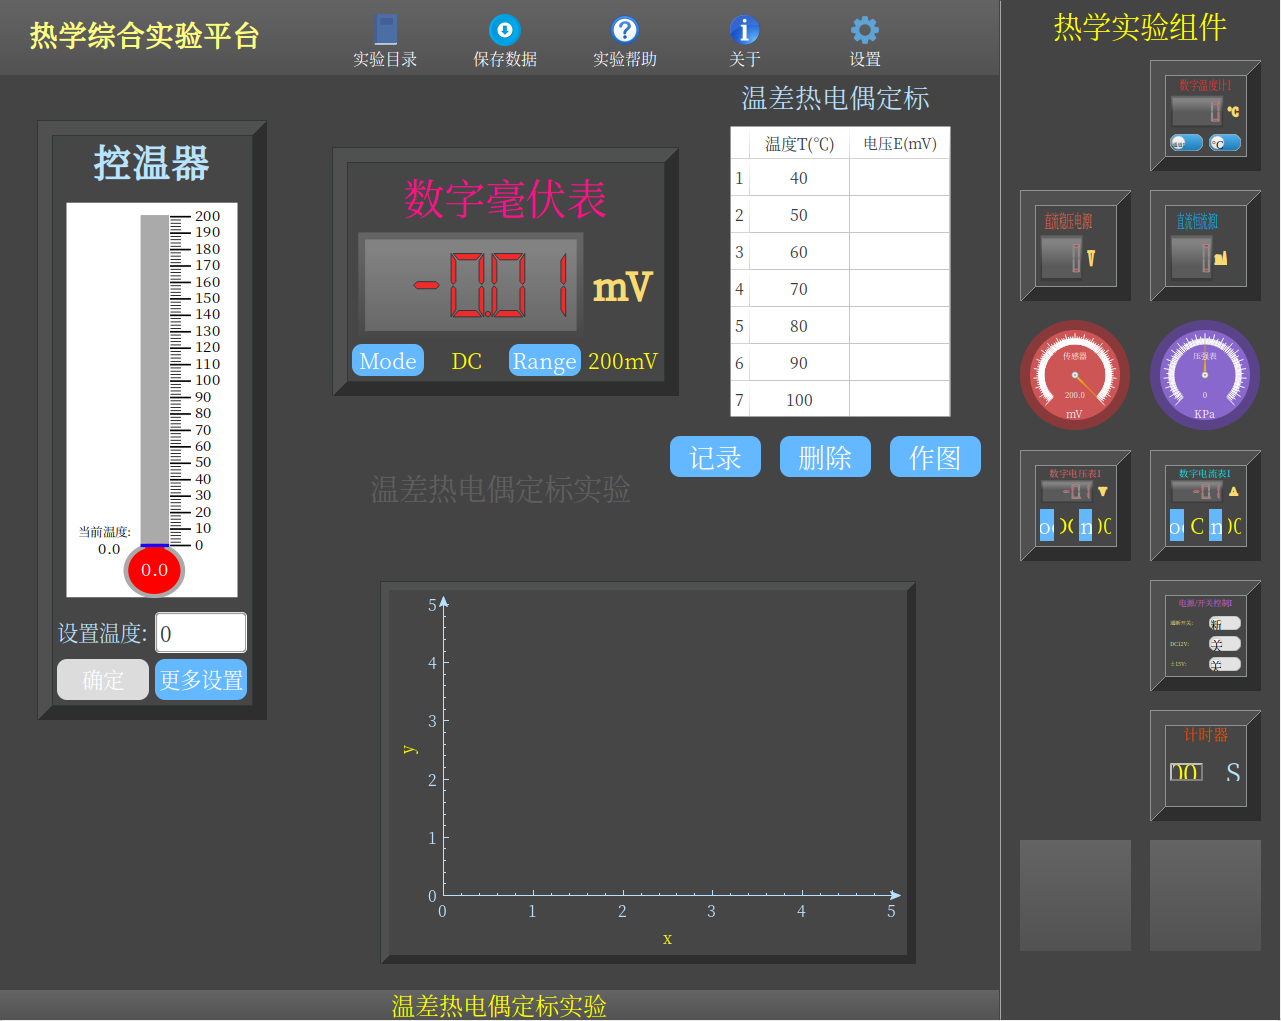
\includegraphics[width=\linewidth]{assets/平台界面.png}
    \caption{实验平台界面}
  \end{minipage}
\end{figure}

实验所用主要器材包括热学综合实验平台、双端热电偶传感器、保温杯、加热井和冰水混合物。

\section{实验原理}

\subsection{热电偶的定义、应用和分类}
热电偶是将两种不同导体或半导体材料连接成回路后，利用两接点温度不同所产生的热电动势来进行测温的传感元件。它把温度这一非电量转化为电压信号进行测量，属于非电量电测法。热电偶具有结构简单、响应较快、测温范围宽、便于远距离传输和记录等优点，因此在工业测温、自动控制、科研实验和日常设备中都有广泛应用。

按用途可将热电偶分为标准热电偶和工作热电偶；按材料组成又可分为多种不同分度号的热电偶。不同材料的热电偶适用温区和灵敏度不同，因此在实际测量前通常需要定标，建立该热电偶输出电动势与温度之间的对应关系。

\subsection{热电效应与热电偶}
热电偶测温的物理基础是热电效应。将两种不同导体 $A$ 和 $B$ 首尾连接成闭合回路，若两个接点温度不同，则回路中会产生热电动势；接触被测对象的一端称为热端或测量端，另一端称为冷端或参考端。热电偶正是利用热端与冷端之间的温差，将温度差转换为可测的电压信号。

\begin{figure}[htbp]
  \centering
  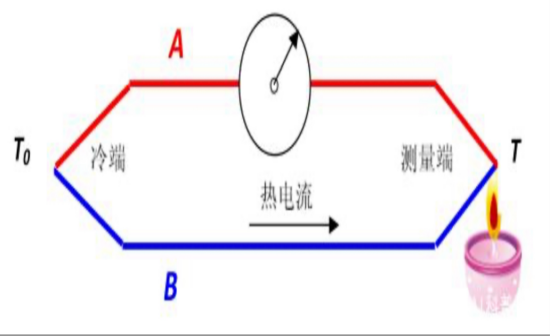
\includegraphics[width=0.58\linewidth]{assets/热电偶原理示意.png}
  \caption{热电偶测温原理示意图}
\end{figure}

热电偶的总热电动势主要由接触电动势和温差电动势组成。两种不同导体接触时，由于材料内部自由电子密度和逸出功不同，界面处会形成电势差，这一部分称为接触电动势；而同一种导体两端温度不同时，热端电子平均动能较大，电子会从高温端向低温端扩散，从而建立温差电动势。二者共同决定热电偶的输出电势。

当热电偶材料确定后，总热电动势主要取决于热端温度 $T$ 与冷端温度 $T_0$。在一定温度范围内，可近似认为热电动势与温差成线性关系：
\[
  E(T,T_0) \approx c(T-T_0),
\]
其中 $c$ 为热电偶的温差系数，其大小由热电偶材料决定。若实验中将冷端置于冰水混合物中，则可近似认为 $T_0=0\,^{\circ}\mathrm{C}$，此时热电动势与热端温度近似成正比。

\subsection{热电偶的定标}
热电偶定标的目的是建立电动势与温度之间的定量关系，以便后续利用电势反推出待测温度。常用的定标方法包括比较法和固定点法。比较法是将被校热电偶与标准热电偶同时测量同一温度，通过对比得到校准关系；固定点法则是利用已知温度点测量热电偶输出电动势，再建立标准曲线。

本实验采用固定点法进行热电偶定标。实验中改变加热井的设定温度，使热端分别处于 $40\,^{\circ}\mathrm{C}$、$50\,^{\circ}\mathrm{C}$、$60\,^{\circ}\mathrm{C}$、$70\,^{\circ}\mathrm{C}$、$80\,^{\circ}\mathrm{C}$、$90\,^{\circ}\mathrm{C}$ 和 $100\,^{\circ}\mathrm{C}$ 等已知温度点，同时保持冷端条件不变。对每个温度点测量对应的热电动势 $E(T)$，即可得到一组 $E(T)$ 与 $T$ 的对应数据。以温度 $T$ 为横轴、热电动势 $E(T)$ 为纵轴作图，并进行线性拟合，就可得到该热电偶在本实验温区内的定标曲线。

\section{实验内容和步骤}

\begin{experimentsteps}
  \item 按图示组装好仪器，连接热学综合实验平台、热电偶传感器、毫伏测量端口和冷端保温杯，检查无误后打开实验平台电源。
  \item 在平台界面上，点击“实验目录”，选择“温差热电偶定标实验”，再从右侧“热学实验组件”中拖出控温器、毫伏表和图像模块。
  \item 调节控温器“设置温度”为 $40\,^{\circ}\mathrm{C}$，点击“确定”完成设定。待系统加热到设定温度并稳定后，点击数据记录表格下方的“记录”按钮，将毫伏表读数记录到表 \ref{table:calibration} 中。
  \item 重复步骤 3，依次将设定温度调整为 $50\,^{\circ}\mathrm{C}$、$60\,^{\circ}\mathrm{C}$、$70\,^{\circ}\mathrm{C}$、$80\,^{\circ}\mathrm{C}$、$90\,^{\circ}\mathrm{C}$ 和 $100\,^{\circ}\mathrm{C}$，在冷端条件保持不变的情况下，记录各温度点对应的热电动势。
  \item 点击平台上的“作图”按钮，观察热电偶的 $E(T)$--$T$ 定标曲线。完成阶段再根据保存的数据整理图线、进行拟合并补充分析。
\end{experimentsteps}

\newcolumntype{Y}{>{\centering\arraybackslash}X}

\begin{LabRecordTable}
  \centering
  \caption{热电偶温度电势记录表}
  \label{table:calibration}
  \renewcommand{\arraystretch}{1.25}
  \setlength{\tabcolsep}{3.5pt}
  \begin{tabularx}{\textwidth}{c *{7}{Y}}
    \toprule
    温度 $T$/\si{\celsius} & 40 & 50 & 60 & 70 & 80 & 90 & 100 \\
    \midrule
    电动势 $E(T)$/\si{\milli\volt} & 1.2 & 1.4 & 1.7 & 2.0 & 2.3 & 2.6 & 2.8 \\
    \bottomrule
  \end{tabularx}
\end{LabRecordTable}

\section{实验数据处理}

根据表 \ref{table:calibration} 中的数据，以温度 $T$ 为横轴、热电动势 $E(T)$ 为纵轴作出热电偶的定标曲线，如图 \ref{fig:calibration} 所示。

\begin{figure}[htbp]
  \centering
  \begin{tikzpicture}
    \begin{axis}[
      width=0.82\textwidth,
      height=0.52\textwidth,
      xlabel={$T / \si{\celsius}$},
      ylabel={$E(T) / \si{\milli\volt}$},
      xmin=38, xmax=102,
      ymin=1.1, ymax=2.9,
      xtick={40,50,60,70,80,90,100},
      ytick={1.2,1.4,1.6,1.8,2.0,2.2,2.4,2.6,2.8},
      grid=both,
      tick label style={font=\small},
      label style={font=\small},
      legend style={font=\small, at={(0.5,-0.16)}, anchor=north, fill=white, draw=none},
      clip=false
    ]
      \addplot[only marks, mark=*, blue] coordinates {
        (40,1.2) (50,1.4) (60,1.7) (70,2.0) (80,2.3) (90,2.6) (100,2.8)
      };
      \addlegendentry{实验数据}
      \addplot[red, domain=40:100, samples=2] {0.027857142857*x + 0.05};
      \addlegendentry{线性拟合}
    \end{axis}
  \end{tikzpicture}
  \caption{热电偶 $E(T)$--$T$ 定标曲线}
  \label{fig:calibration}
\end{figure}

采用最小二乘法进行线性拟合，可得该热电偶在本实验温区内的定标方程为
\[
  E(T) = 0.02786T + 0.05000,
\]
其中 $E$ 的单位为 \si{\milli\volt}，$T$ 的单位为 \si{\celsius}。拟合的决定系数为
\[
  R^2 = 0.9967,
\]
线性相关系数为
\[
  r = 0.9984.
\]
由此可见，在 $40\,^{\circ}\mathrm{C}$ 至 $100\,^{\circ}\mathrm{C}$ 的实验范围内，热电动势与温度呈显著线性正相关关系。由拟合直线斜率可得该热电偶在本实验条件下的灵敏度约为
\[
  c = 0.02786\ \si{\milli\volt\per\celsius}
  = 27.86\ \si{\micro\volt\per\celsius}.
\]

若以后需要由电动势反推出温度，可将上式改写为
\[
  T = 35.897E - 1.795,
\]
其中 $E$ 的单位仍取 \si{\milli\volt}。该式可作为本实验所用热电偶在相同冷端条件下的近似定标公式。

\section{实验的分析和总结}

由图 \ref{fig:calibration} 可见，实测点基本分布在同一直线附近，且电动势随温度升高单调增大，说明该热电偶在本实验温区内满足较好的线性响应规律。平均来看，温度每升高 $10\,^{\circ}\mathrm{C}$，热电动势约增加 $0.279\,\si{\milli\volt}$。拟合截距仅为 $0.050\,\si{\milli\volt}$，相对于实验测得的 $1.2$--$2.8\,\si{\milli\volt}$ 而言较小，表明定标曲线与理想情况下过原点的线性关系较为接近。

本实验的误差主要可能来自以下几个方面。首先，冷端虽然置于冰水混合物中，但其温度未必始终严格保持在 $0\,^{\circ}\mathrm{C}$，冷端温度的微小漂移会直接影响热电动势读数。其次，各设定温度点若尚未完全稳定就读取毫伏表，热端实际温度与设定温度之间可能存在偏差。再次，毫伏表分辨率、人工记录时的读数误差以及热电偶与加热井、引线端接触不良，都可能使某些数据点相对拟合直线产生轻微偏离。此外，环境散热和导线附加热电势也会带来一定系统误差。

若冷端不处于冰水混合物中，而是位于实际温度 $T_0$，则实测电动势记为 $E_{\mathrm{m}}$，它反映的是热端与冷端之间的温差效应。根据冷端补偿思想，应先求出冷端温度对应的补偿电动势
\[
  E(T_0,0) = 0.02786T_0 + 0.05000,
\]
再与实测值相加，得到相对于 $0\,^{\circ}\mathrm{C}$ 冷端的等效电动势
\[
  E_{\mathrm{c}} = E_{\mathrm{m}} + E(T_0,0).
\]
随后代入定标方程
\[
  T = 35.897E_{\mathrm{c}} - 1.795
\]
即可求出热端温度。若仍采用本实验得到的线性近似，则上式可进一步化简为
\[
  T \approx 35.897E_{\mathrm{m}} + T_0.
\]
因此，冷端补偿的本质是把非 $0\,^{\circ}\mathrm{C}$ 冷端造成的缺失电动势补回去，再利用定标曲线反算热端温度。

\insertSignedDataPage

\end{document}
